\documentclass[tikz, margin=3mm]{standalone}
\usetikzlibrary{chains, positioning}

\begin{document}
    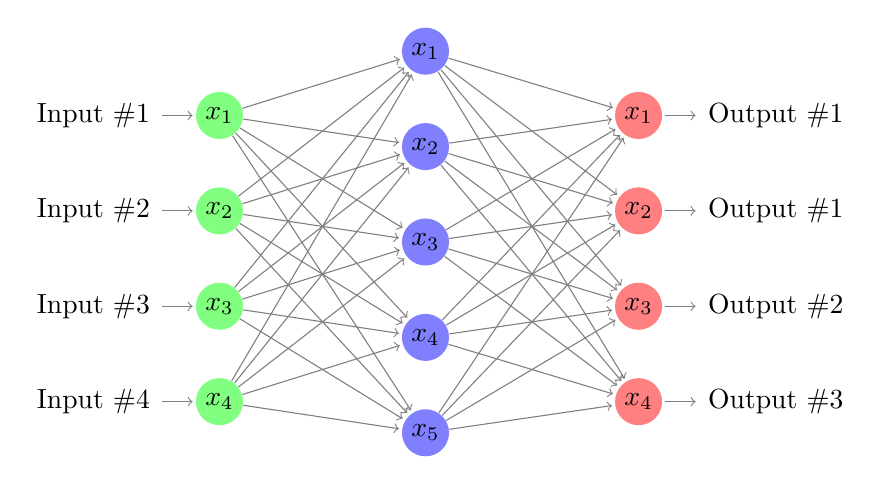
\begin{tikzpicture}[shorten >=1pt,->, draw=black!50, 
        node distance = 6mm and 24mm,
          start chain = going below,
every pin edge/.style = {<-,shorten <=1pt},
        neuron/.style = {circle, fill=#1, 
                         minimum size=17pt, inner sep=0pt,
                         on chain},
         annot/.style = {text width=4em, align=center}
                        ]
% Draw the input layer nodes
\foreach \i in {1,...,4}
    \node[neuron=green!50,
          pin=180:Input \#\i] (I-\i)    {$x_{\i}$};
% Draw the hidden layer nodes
    \node[neuron=blue!50,
          above right=6mm and 24mm of I-1.center] (H-1)     {$x_{1}$};
\foreach \i [count=\j from 1] in {2,...,5}
    \node[neuron=blue!50,
          below=of H-\j]      (H-\i)    {$x_{\i}$};
% Draw the output layer node
    \node[neuron=red!50,
          pin= {[pin edge=->]0:Output \#1},
          right=of I-1 -| H-1]  (O-1)   {$x_{1}$};
\foreach \i [count=\j from 1] in {2,...,4}
    \node[neuron=red!50,
          pin= {[pin edge=->]0:Output \#\j},
          below=of O-\j]        (O-\i)  {$x_{\i}$};
% Connect input nodes with hidden nodes and 
%  hiden nodes with output nodes with the output layer
    \foreach \i in {1,...,4}
        \foreach \j in {1,...,5}
{
    \path (I-\i) edge (H-\j)
          (H-\j) edge (O-\i);
}
    \end{tikzpicture}
\end{document}
